\documentclass{article}

\PassOptionsToPackage{numbers, compress}{natbib}
\usepackage[sglblindworkshop, final]{neurips_2026}
\workshoptitle{Machine Learning for Systems}

\usepackage[utf8]{inputenc}
\usepackage[T1]{fontenc}
\usepackage{hyperref}
\usepackage{url}
\usepackage{booktabs}
\usepackage{amsmath}
\usepackage{amsfonts}
\usepackage{microtype}
\usepackage{graphicx}
\graphicspath{{../figures/}}

\title{Which Eviction Policy Should an LLM Cache Use?\\
A Systematic Study Across Workloads, Capacities, and Encoders}

\author{%
  Yash Kulkarni \\
  University of Michigan\\
  \texttt{yashkulk@umich.edu}
  \And
  Shubham Harkare \\
  University of Michigan\\
  \texttt{sharkare@umich.edu}
  \And
  Arvind Suresh Yogesh Babu \\
  University of Michigan\\
  \texttt{savyo@umich.edu}
}

\begin{document}

\maketitle

\begin{abstract}
Semantic caches answer an incoming query with the response stored for a nearby
embedding, but proposed eviction policies have not been compared under one
protocol. We evaluate FIFO, LRU, LFU, ARC, GDSF, a streaming adaptation of
SISO, and a semantic-redundancy policy across three ordered query corpora,
three cache capacities, and two encoders. No evaluated policy improves on LFU
by more than 0.0409 percentage points in any of the eighteen settings.
Replacement still matters at tight capacity: FIFO and streaming SISO trail LFU
by as much as 8.7 points. We explain the missing upside with a conditional
packing result. Under exact lookup and insert-on-miss, a newly inserted entry
cannot have a resident neighbor within the hit radius, so a geometry-aware
eviction rule receives little new redundancy signal. A separate audit finds a
larger problem. At a median-nearest-neighbor operating point, only 2.1--3.9\%
of sampled LMSYS and QQP hits are judged answer-substitutable, reducing raw
hit rates of 51--60\% to quality-adjusted rates of 1.1--2.2\%. LFU is the
strongest simple default in this protocol, but threshold calibration and hit
validity require attention before sub-point eviction differences.
\end{abstract}

\section{Introduction}
A semantic cache embeds an LLM request and reuses a stored response when the
nearest cached query falls within a distance threshold
\citep{bang2023gptcache}. Classical policies such as LRU and LFU compete with
ARC \citep{megiddo2003arc}, GDSF \citep{cherkasova1998gdsf}, and policies that
use embedding geometry \citep{kim2025siso,liu2026semantic,sun2026solar}.
Published orderings differ. Sun et al.\ \citep{sun2026solar}, for example,
report FIFO beating LRU and LFU on agent-memory workloads.

We compare seven policies while holding the query order, index, threshold, and
measurement suffix fixed. The result is narrower than ``eviction does not
matter.'' No complex policy improves meaningfully on LFU, but poorly matched
policies can lose several points. We also identify when semantic redundancy is
suppressed by insert-on-miss admission and test whether the nominal hits are
safe response reuses.

\section{Study design}
\label{sec:design}
\textbf{Inputs.} We form 100K-query corpora from the first user utterance in
each LMSYS-Chat-1M conversation \citep{zheng2023lmsys}, individual Quora
Question Pairs questions \citep{iyer2017qqp}, and MOSS instructions
\citep{sun2024moss}. Preprocessing removes exact duplicate text. We sample
without replacement and restore source-row order. These inputs preserve corpus
order but are not request traces; in particular, they contain no exact query
repetition. We test capacities of 10\%, 20\%, and 30\% under MiniLM
\citep{reimers2019sbert} and gte-base \citep{li2023gte}.

\textbf{Cache protocol.} A nearest neighbor within the hit threshold is served
without insertion; a miss is inserted and may trigger eviction. The cache uses
FAISS HNSW ($M{=}32$, $\mathit{efConstruction}{=}128$,
$\mathit{efSearch}{=}128$). For a capacity fraction $C$, we prefill the cache
with the first $C$ of the corpus, exclude the remainder of the first 30\%, and
measure the final 70\%. Thus every capacity sees the same measured suffix, but
the protocol is a capacity-sized prefill rather than a 30\% online warmup.
MiniLM uses $L_2^2 \leq 0.90$ (cosine $\geq 0.55$ for unit vectors), its
median-nearest-neighbor operating point; gte-base parameters are matched by
empirical similarity quantile.

\textbf{Policies and repetitions.} We test FIFO, LRU, LFU, ARC, GDSF, a
single-pass streaming adaptation of SISO \citep{kim2025siso}, and a semantic
policy that ranks redundancy relative to recency-frequency utility. Three
seeds vary randomized policy-side sampling; they do not create independent
traces. The maximum standard deviation over the 126 policy cells is
$3.1\times10^{-4}$ in hit-rate units.

\textbf{Hit audit.} At 10\% capacity under MiniLM, we sample 1{,}000 hits per
dataset-policy cell across distance quantiles, producing 13{,}669 unique
pairs. A Llama-3.1-8B judge \citep{grattafiori2024llama} asks whether a
correct, complete answer to the cached query would also answer the incoming
query. We call a YES verdict \emph{answer-substitutable}. Rejudging 1{,}931
pairs with a second runtime serving the same model family gives 98.55\%
agreement ($\kappa=0.826$); this checks runtime consistency, not human
validity.

\section{Results}
\subsection{No complex policy improves on LFU}
\label{sec:matrix}
Figure~\ref{fig:heatmap} reports the matrix. The largest gain over LFU is
0.0409\,pp. ARC remains within 0.01\,pp of LFU, GDSF follows LFU-with-aging,
and the semantic policy adds $3.4$--$5.9\times$ LRU's per-query time on LMSYS
and QQP without a larger hit rate.

The weak policies show why the conclusion must stay bounded. FIFO never beats
LRU and ranks sixth or seventh in seventeen of the eighteen cells; the
exception is a saturated MOSS cell where all seven policies lie within
0.012\,pp. Streaming SISO and FIFO
differ by 0.096\,pp on average across LMSYS and QQP, but streaming SISO trails
LFU by up to 8.55\,pp and costs $2.8$--$5.3\times$ LRU on those corpora. These are descriptive
comparisons on one ordered corpus per dataset, not significance tests across
request traces. They do not reproduce Sun et al.'s FIFO ordering
\citep{sun2026solar}; differences in repetition, locality, cache semantics, or
implementation remain hypotheses until tested in one shared workload.

Capacity narrows rather than eliminates every gap. LFU's lead over LRU falls
from 1.5\,pp on LMSYS and 2.5\,pp on QQP at 10\% capacity to at most
0.012\,pp at 30\%; the largest streaming-SISO deficit at 30\% is still
1.40\,pp.

\begin{figure}[t]
  \centering
  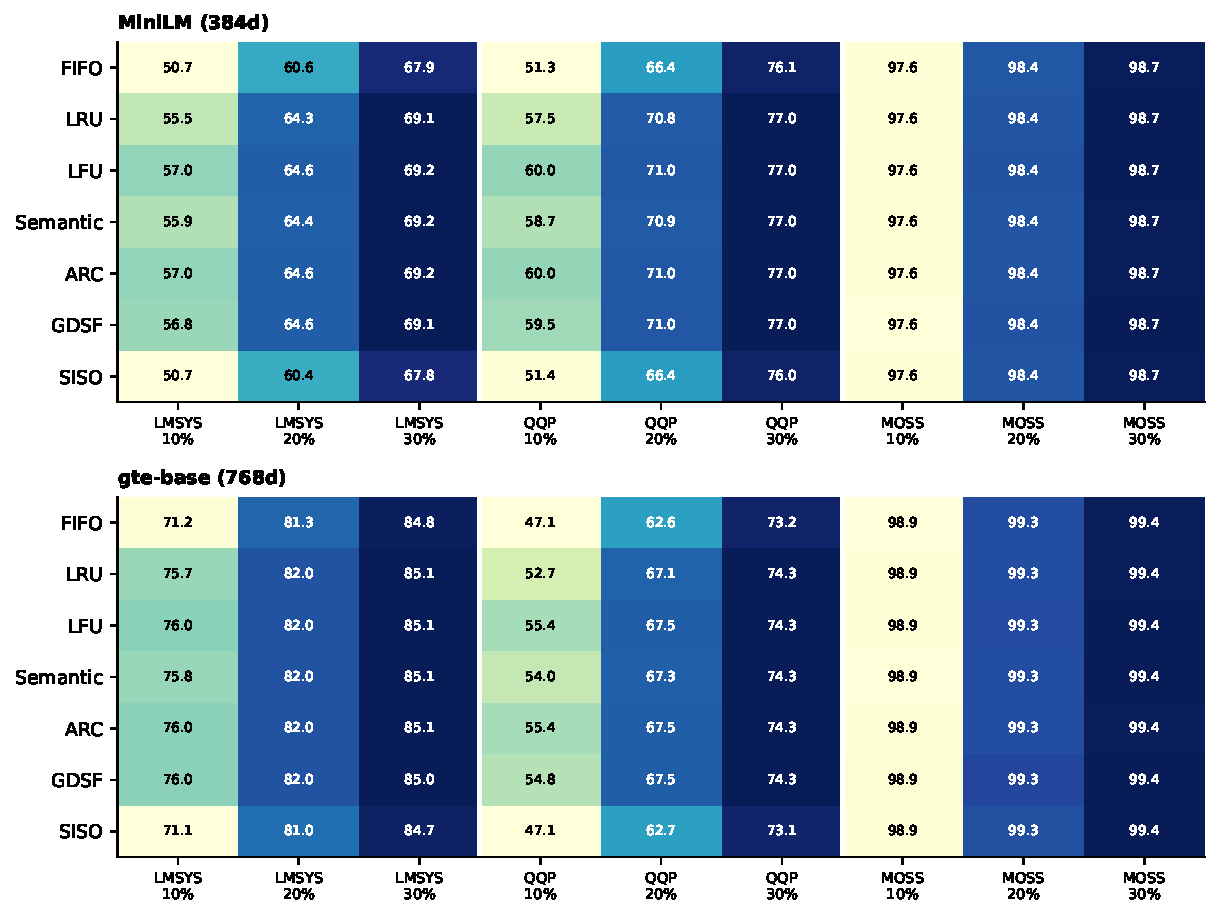
\includegraphics[width=0.9\linewidth]{phase6_policy_heatmap}
  \caption{Hit rate (\%) by policy, corpus, capacity, and encoder; color is
  normalized within each corpus block. No policy improves on LFU by more than
  0.0409\,pp, while FIFO and streaming SISO lose several points at tight
  capacity.}
  \label{fig:heatmap}
\end{figure}

\subsection{The operating point matters more than the winner}
\label{sec:encoders}
Using MiniLM's threshold unchanged with gte-base makes every measured request a
hit and produces zero evictions. After matching thresholds by similarity
quantile, the leading-policy ordering returns, but LFU's absolute hit rate
moves by $+19.0$\,pp on LMSYS and $-4.6$\,pp on QQP. A threshold is therefore
an encoder-specific operating point, and distribution matching does not
establish response quality.

Figure~\ref{fig:qadj} tests that quality directly. Answer-substitutable
fractions are 3.1--3.9\% on LMSYS and 2.1--3.1\% on QQP. Their Wilson
intervals overlap across policies, while quality-adjusted hit rates fall to
1.1--2.2\%. Even LMSYS's nearest distance decile, with median
$L_2^2=0.10$, reaches only 8.9\% YES. Shared prompt templates often hide
different payloads. The measured threshold is useful for stressing eviction,
not suitable as a deployment recommendation. Verified caching reaches a
related design conclusion \citep{schroeder2025vcache}.

\begin{figure}[t]
  \centering
  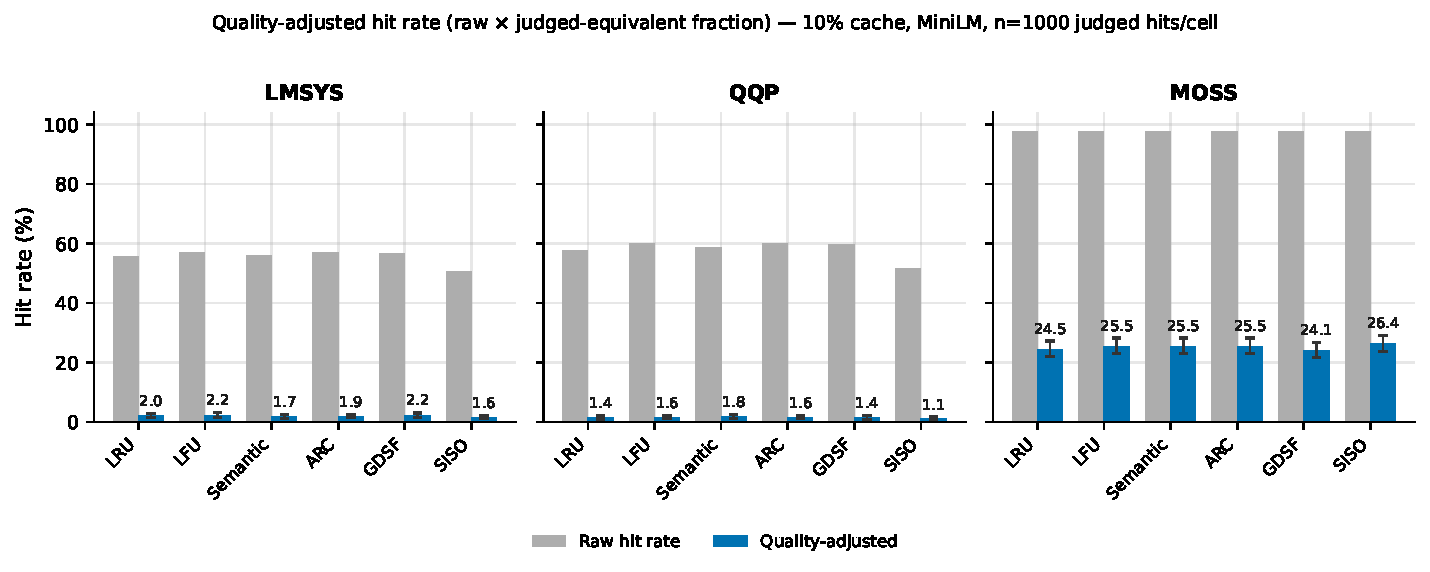
\includegraphics[width=0.9\linewidth]{judge_quality_adjusted}
  \caption{Raw and answer-substitutability-adjusted hit rate at 10\% capacity
  under MiniLM (Wilson 95\% intervals). The audited operating point admits
  few reusable LMSYS and QQP pairs.}
  \label{fig:qadj}
\end{figure}

\section{Why semantic signal disappears}
\label{sec:mechanism}
\textbf{Packing condition.} Let $C_t$ be the resident embeddings before query
$q_t$, and let $h$ be the hit radius. With exact lookup and insert-on-miss,
$q_t$ is inserted only if $\min_{c\in C_t} d(q_t,c)>h$. For any redundancy
radius $r\leq h$, the inserted entry therefore has no redundancy edge to any
resident entry, and every later insertion satisfies the same condition, so two
stream-inserted entries are never within $r$ of each other while both are
resident. The claim does not
cover arbitrary prefill contents, approximate-search false misses, insertion
on hits, or policies that move stored representations.

Our density profile is consistent with this condition but does not prove it
across the matrix. In the 10\%-capacity MiniLM LRU cache, the mean
within-threshold neighbor fraction at the end of the measured stream is
$2.1\times10^{-5}$ for QQP,
$4.1\times10^{-4}$ for LMSYS, and $2.5\times10^{-3}$ for MOSS. The largest
value is $40\times$ below the semantic policy's smoothing constant
$\mu=0.1$, so redundancy contributes little to its ranking in this
configuration.

\section{Decision and validity limits}
For an insert-on-miss cache under this protocol, LFU is the strongest simple
default. Teams considering semantic eviction should first measure resident
cache density at the intended hit radius. More importantly, they should set
that radius against human-validated answer substitutability, not an embedding
quantile alone.

Four limits constrain the ranking. Exact duplicate removal means the corpora
do not measure repeated requests. The prefill protocol omits part of the first
30\% and is not a continuous warmup. The common HNSW index controls the policy
comparison, but its separately measured 2.2\,pp static Recall@1 loss exceeds
the differences among the leading policies; approximate misses also change
later cache state, so exact-index replication is needed before interpreting
sub-point ranks. Finally, the audit uses one 8B judge family, one encoder, one
capacity, and six policies, without human labels or stored responses. Under
these limits, LFU is preferable to the added policy complexity tested here;
eviction is not universally irrelevant.

\begin{ack}
This work was conducted as part of CSE 584 (Advanced Database Systems) at the University of Michigan. We thank Lin Ma for guidance and feedback, and the University of Michigan Great Lakes HPC cluster for compute. The authors declare no competing interests.
\end{ack}

\bibliographystyle{plain}
\bibliography{../../references}

\appendix

\section{Judge rubric and validation}
The judge is Llama-3.1-8B-Instruct served locally via Ollama at temperature 0
with a 16-token completion cap. The user prompt asks: ``Would a correct,
complete answer to the ORIGINAL question also be a correct and complete answer
to the NEW question? Reply with exactly one word: YES or NO.'' 13{,}667 of
13{,}669 pairs parse. This directional test measures answer substitutability,
not symmetric query equivalence. QQP has no stored answers, so we could not
perform a response-grounded audit. The 1{,}931-pair overlap between local
Ollama and Groq's hosted llama-3.1-8b-instant, using the same rubric, gives
98.55\% agreement and $\kappa=0.826$. Because both runtimes serve the same
model family, this result measures consistency rather than correctness.

\section{Per-encoder recalibration}
MiniLM's hit threshold of $0.90$ $L_2^2$ (cosine $0.55$) is its median
nearest-neighbor similarity over the 100K-query corpora. For gte-base, the hit
and redundancy thresholds become $0.30$ $L_2^2$ (cosine $0.85$), the
streaming-SISO clustering threshold moves from cosine $0.86$ to $0.94$, and ARC's
ghost-match threshold moves from $0.20$ to $0.10$ $L_2^2$. Non-geometric
parameters are unchanged. This in-sample distribution calibration makes the
matrix non-degenerate; it is neither held-out calibration nor evidence that
the resulting hits are valid.

\section{Reproducibility}
Every run writes a JSON manifest with its command line, config hash, package
versions, Git commit, and host hardware. Eviction cells use seeds
\{42, 123, 456\}; the judge sample uses seed 42. The semantic policy sets
$\alpha=\beta=1.0$, $\mu=0.1$, $\varepsilon=10^{-9}$, and caps neighbor
sampling at 1{,}024. At 10\% capacity, per-query cost relative to LRU is
$4.3\times$ (LMSYS) and $3.8\times$ (QQP) for the semantic policy, and
$3.5\times$ and $3.1\times$ for streaming SISO.

\end{document}
